\chapter{Results}\label{chapter:results}

This chapter presents the results of the experiments conducted to evaluate the performance of the different setups.

\section{Vocabulary Statistics}
\begin{figure}[H]
    \centering
    \begin{subfigure}[b]{0.48\linewidth}
        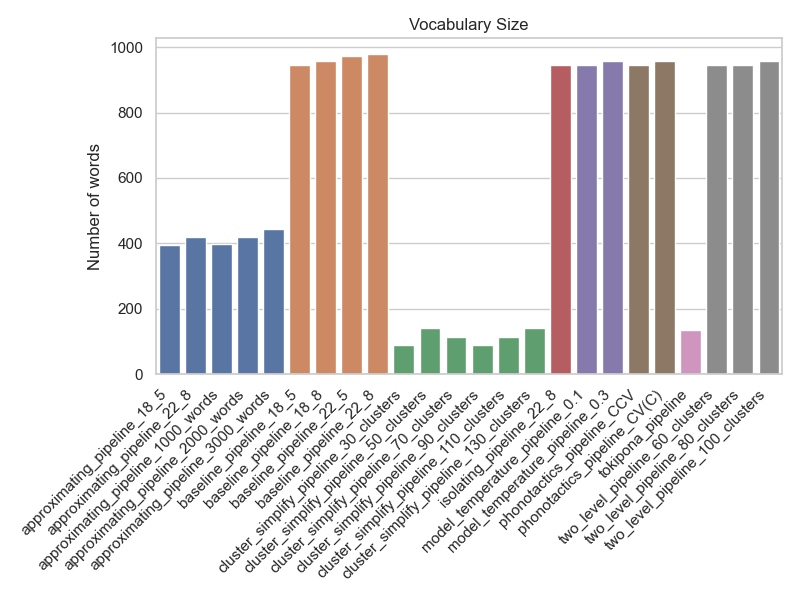
\includegraphics[width=\linewidth]{figures/results/vocabulary_size.png}
        \caption{Vocabulary Size}
        \label{fig:vocabulary-size}
    \end{subfigure}
    \hfill
    \begin{subfigure}[b]{0.48\textwidth}
        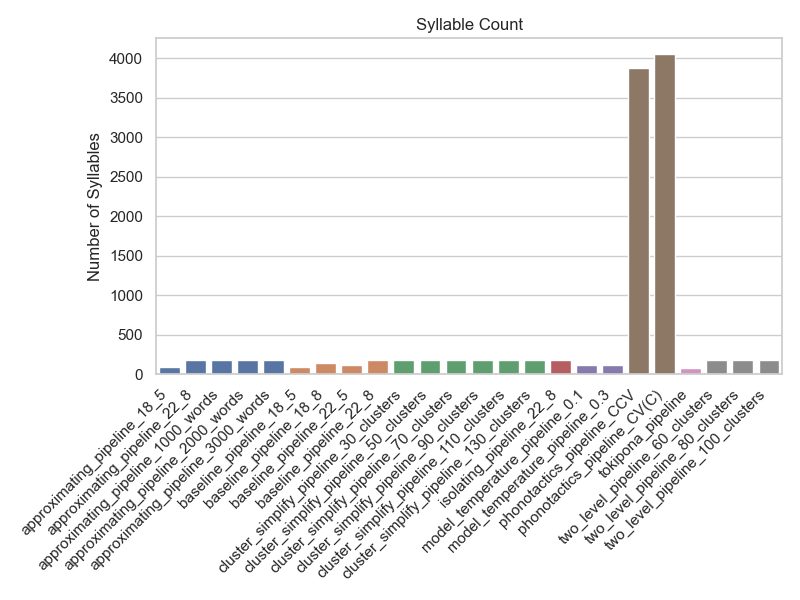
\includegraphics[width=\linewidth]{figures/results/syllable_count.png}
        \caption{Syllable Count}
        \label{fig:syllable-count}
    \end{subfigure}
    \caption{Vocabulary Statistics.}
    \label{fig:vocabulary-statistics}
\end{figure}

Figure \ref{fig:vocabulary-statistics} shows the vocabulary size and syllable count for each setup. 
The vocabulary size is the number of unique words generated, while the syllable count is the total number of possible syllables in the language. 
The approximating and cluster simplify strategies have the smallest vocabulary size, along with Toki Pona. Syllable counts are based on the total number of phonemes and 
the phonotactic rules, and so the phonotactics pipeline has the highest syllable count by far.

\section{Bert Evaluation}

\begin{figure}[H]  
    \centering
    \begin{subfigure}[b]{0.48\linewidth}
        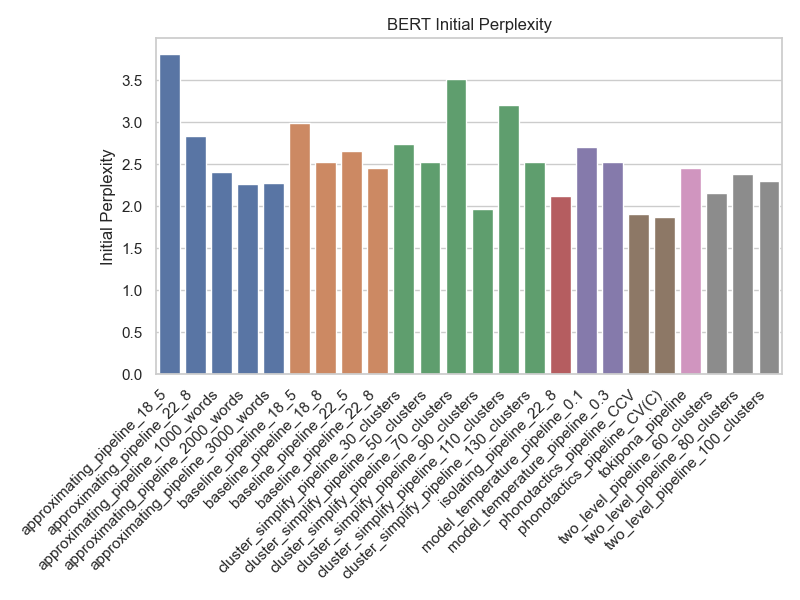
\includegraphics[width=0.7\linewidth]{figures/results/bert_initial_perplexity.png}
        \caption{BERT Initial Perplexity}
        \label{fig:bert-initial-perplexity}
    \end{subfigure}
    \hfill
    \begin{subfigure}[b]{0.48\linewidth}
        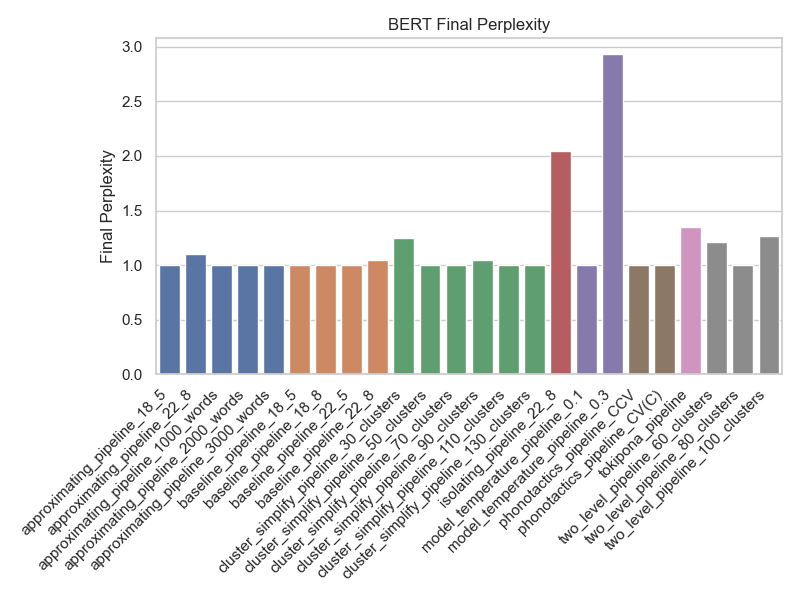
\includegraphics[width=0.7\linewidth]{figures/results/bert_final_perplexity.png}
        \caption{BERT Final Perplexity}
        \label{fig:bert-final-perplexity}
    \end{subfigure}
    
    \begin{subfigure}[b]{0.48\linewidth}
        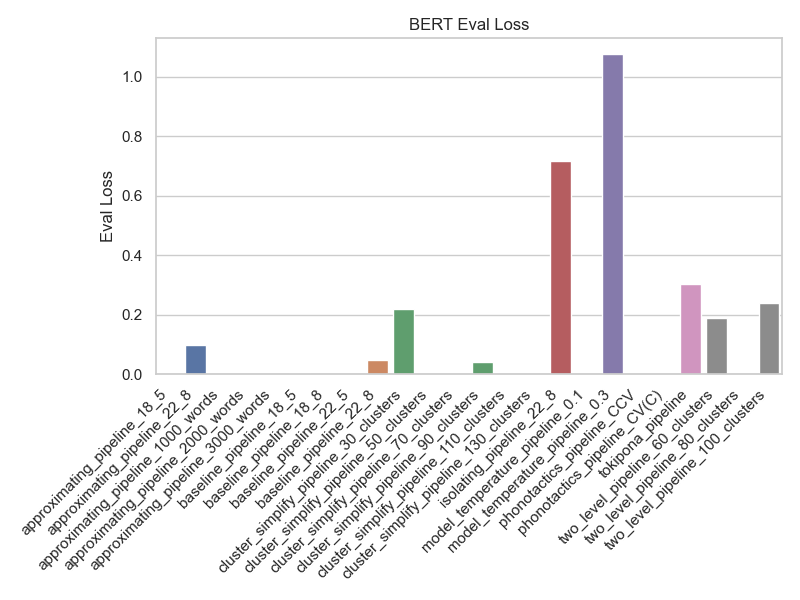
\includegraphics[width=0.7\linewidth]{figures/results/bert_eval_loss.png}
        \caption{BERT Eval Loss}
        \label{fig:bert-eval-loss}
    \end{subfigure}
    \hfill
    \begin{subfigure}[b]{0.48\linewidth}
        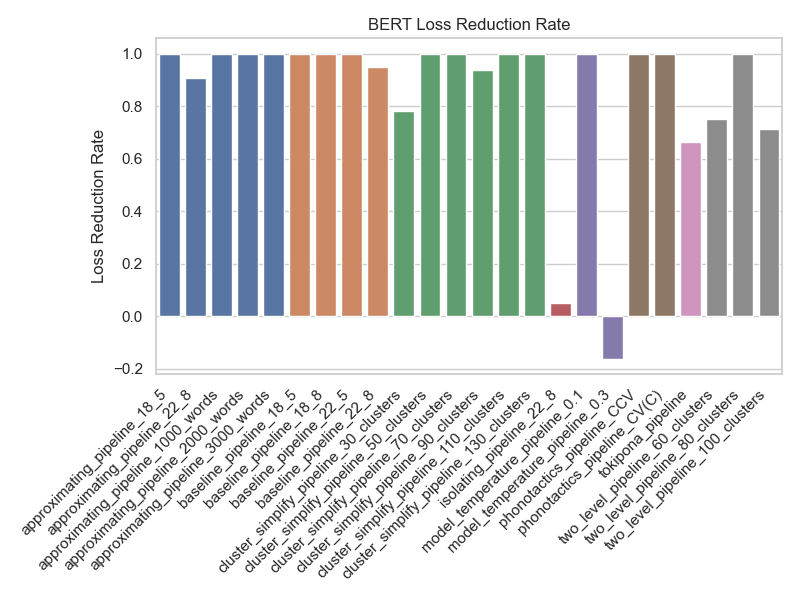
\includegraphics[width=0.7\linewidth]{figures/results/bert_loss_reduction_rate.png}
        \caption{BERT Loss Reduction Rate}
        \label{fig:bert-loss-reduction-rate}
    \end{subfigure}
    \caption{BERT Evaluation}
    \label{fig:bert-statistics}
\end{figure}

Figure \ref{fig:bert-statistics} shows the BERT evaluation results.
The initial perplexity is the perplexity of the model before training, i.e. how confused the model was about predicting masked words, before the fine tuning process.
The final perplexity is the perplexity of the model after training, i.e. how confused the model was about predicting masked words, after the fine tuning process.
The Eval Loss is the final evaluation loss from the model after training, and the loss reduction rate indicates how much the loss was reduced during training.


\section{Translation Scores}

\begin{figure}[H]  
    \centering
    \begin{subfigure}[b]{0.48\linewidth}
        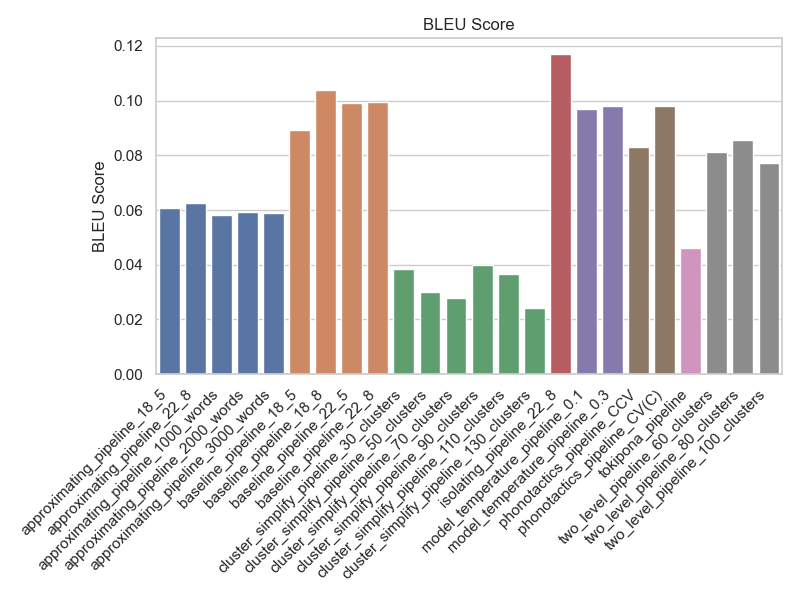
\includegraphics[width=0.7\linewidth]{figures/results/bleu_scores.png}
        \caption{BLEU Scores}
        \label{fig:bleu-scores}
    \end{subfigure}
    \hfill
    \begin{subfigure}[b]{0.48\linewidth}
        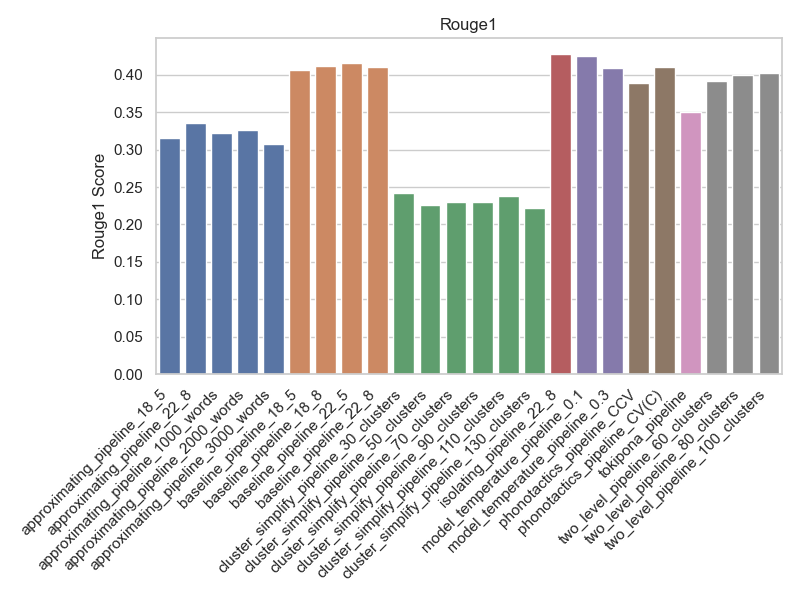
\includegraphics[width=0.7\linewidth]{figures/results/rouge1_scores.png}
        \caption{Rouge 1 Scores}
        \label{fig:rouge1-scores}
    \end{subfigure}

    \begin{subfigure}[b]{0.48\linewidth}
        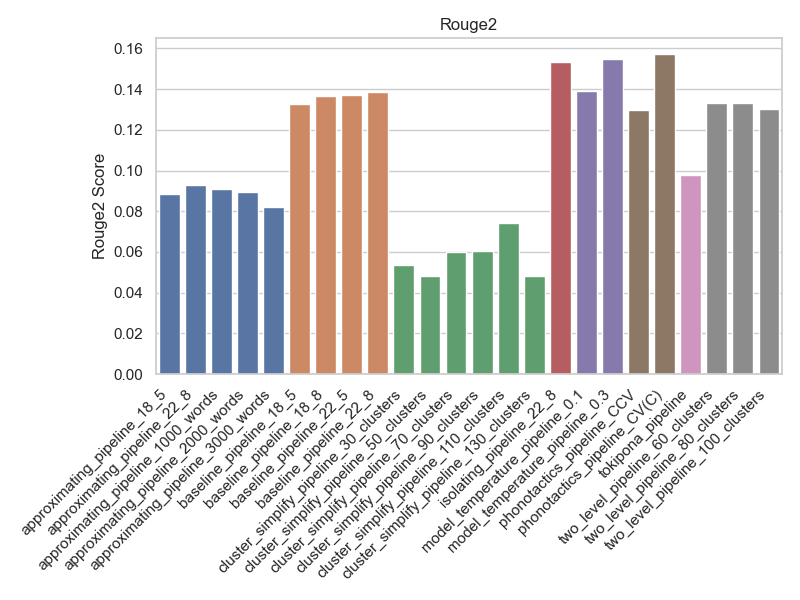
\includegraphics[width=0.7\linewidth]{figures/results/rouge2_scores.png}
        \caption{Rouge 2 Scores}
        \label{fig:rouge2-scores}
    \end{subfigure}
    \hfill
    \begin{subfigure}[b]{0.48\linewidth}
        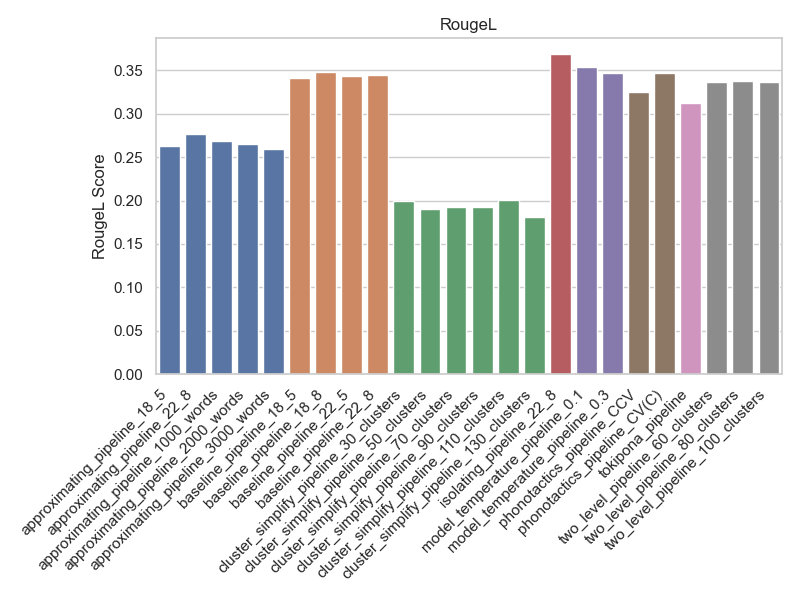
\includegraphics[width=0.7\linewidth]{figures/results/rougeL_scores.png}
        \caption{Rouge L Scores}
        \label{fig:rougel-scores}
    \end{subfigure}

    \begin{subfigure}[b]{0.48\linewidth}
        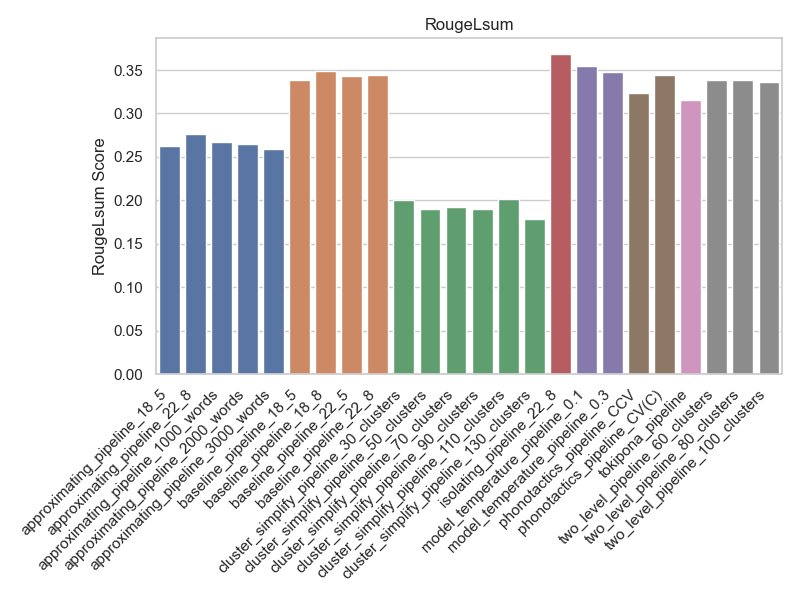
\includegraphics[width=0.7\linewidth]{figures/results/rougeLsum_scores.png}
        \caption{Rouge L Sum Scores}
        \label{fig:rougelsum-scores}
    \end{subfigure}
    \hfill
    \begin{subfigure}[b]{0.48\linewidth}
        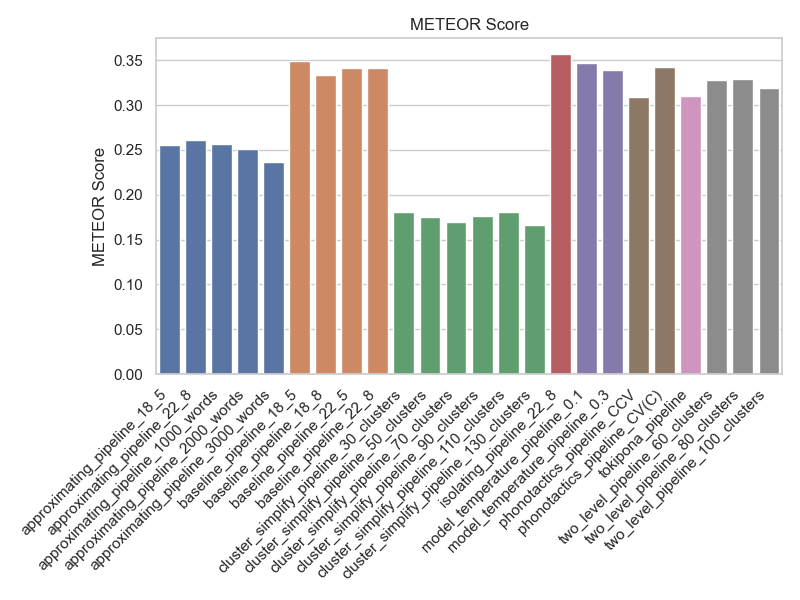
\includegraphics[width=0.7\linewidth]{figures/results/meteor_scores.png}
        \caption{Meteor Scores}
        \label{fig:meteor-scores}
    \end{subfigure}
    \caption{Translation Scores}
    \label{fig:translation-statistics}
\end{figure}

Figure \ref{fig:translation-statistics} shows the translation scores for each setup. Once we translate and then detranslate the source text to and from the constructed language, 
we use the well known BLEU, ROUGE, and METEOR metrics to evaluate the quality of the translation. Higher scores indicate better translation quality.
As we can see, the approximating and cluster simplify strategies have the lowest scores, which makes sense considering there would be some amount of information loss in the process of
simplifying. 

\section{Race-C Evaluation}
\begin{figure}[H]  
    \centering
    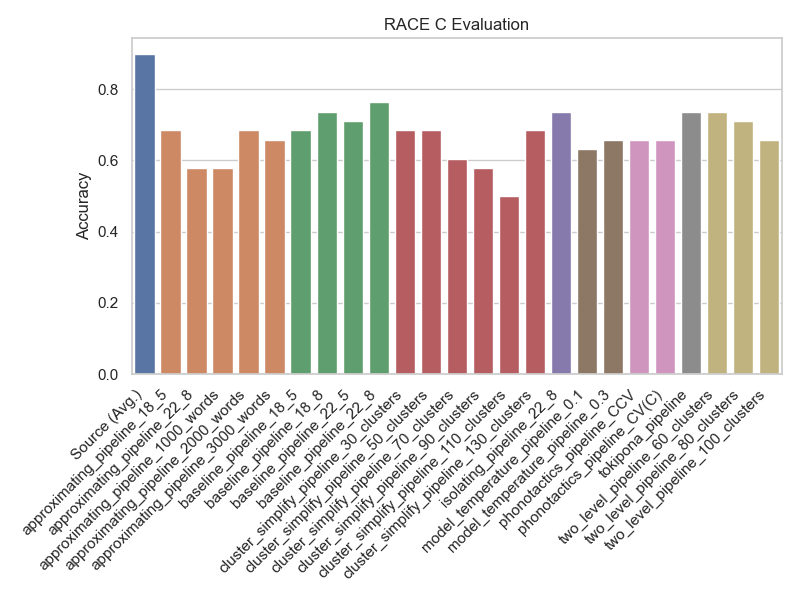
\includegraphics[width=0.7\linewidth]{figures/results/race_c_evaluations.png}
    \caption{Race-C Scores.}
    \label{fig:race-c-scores}
\end{figure}

Figure \ref{fig:race-c-scores} shows how well the model was able to answer the questions from the race-c evaluation, given the source text, or the detranslated
text. As expected, the original text has the highest score. Interestingly, the simplified and approximating pipelines do not perform much less 
than the other pipelines compared to the sharp drop seen in the translation scores.

\section{Zipf's Law Evaluation}
\begin{figure}[H]  
    \centering
    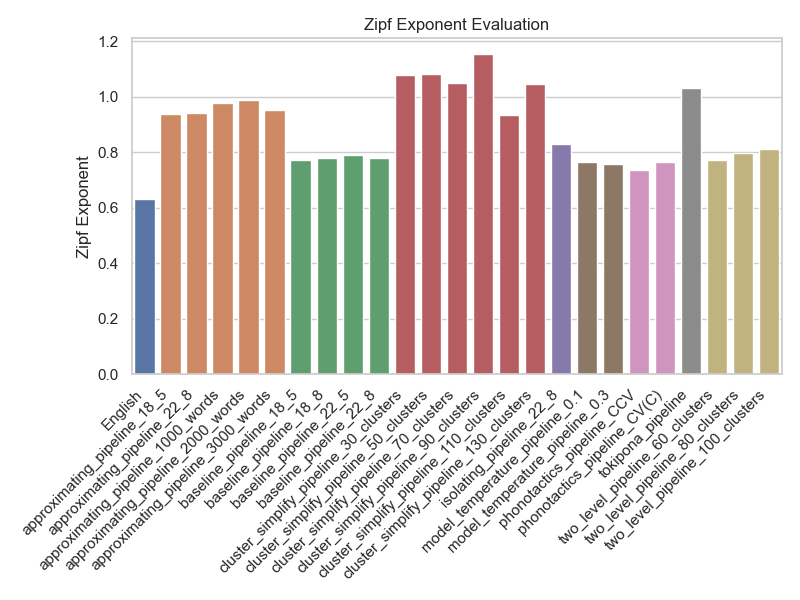
\includegraphics[width=0.7\linewidth]{figures/results/zipfs_law_evaluations.png}
    \caption{Zipf's Exponent}
    \label{fig:zipfs-law-scores}
\end{figure}

Figure \ref{fig:zipfs-law-scores} shows the Zipf's exponent for each setup. The exponent is a measure of how well the word frequency distribution follows Zipf's law,
which states that the frequency of a word is inversely proportional to its rank in the frequency table.
A value of 1 indicates a perfect fit to Zipf's law, while a value of 0 indicates no fit at all. In our case, since the source text we use is small, we expect
some deviation from the law. However, it can still be useful to compare different setups. In this case, we can note that the approximating and cluster simplify strategies
get the closest to the law, along with toki pona. This makes sense, since the chance of rare words appearing in the text is lower, and so the distribution is more uniform.
It also explains why English has such a low exponent, since in such a small text, the chance of rare words appearing is much higher.



